% Sample LaTeX file for creating a paper in the Morgan Kaufmannn two
% column, 8 1/2 by 11 inch proceedings format.

\documentclass{llncs}
\usepackage[margin=1in]{geometry}

% Set the typeface to Times Roman
\usepackage{times}
\usepackage{helvet}
\usepackage{courier}
\usepackage{amssymb}
\usepackage{amsmath}
\usepackage{rotating}
\usepackage{array}
\usepackage{float}
\usepackage{graphics,graphicx,epsfig,epstopdf}
\usepackage{psfrag}
\usepackage{subfigure}
\usepackage{tikz}
\usepackage{url}
\usepackage{color}
\usepackage{theorem}
\usepackage{algorithm}
\usepackage[noend]{algpseudocode}

\usepackage{verbatim}
\usepackage{enumitem}
\usepackage{multirow}
\usepackage{mathabx}
\usepackage{xr}

%\newtheorem{theorem}{Theorem}
%\newtheorem{corollary}{Corollary}[theorem]
%\newtheorem{lemma}[theorem]{Lemma}
%\newtheorem{definition}{Definition}
%\newtheorem{observation}{Observation}
%\newtheorem{example}{Example}
%\newtheorem{problem}{Problem}
%\newtheorem{proposition}{Proposition}
\DeclareMathOperator*{\argmin}{arg\,min}
\DeclareMathOperator*{\argmax}{arg\,max}

\newcommand{\Att}{$\mathcal{A}$}
\newcommand{\Def}{$\mathcal{D}$}

\frenchspacing
\setlength{\pdfpagewidth}{8.5in}
\setlength{\pdfpageheight}{11in}

\title{Approximating the Allocation of Heterogeneous Resources\\to Prevent Illegal Logging}
%\title{Instructions for Authors}

%\title{STEPS: Scaling Techniques for Environmental Protection and Security}
%\title{Simple Heuristics for Allocating Resources against Illegal Loggers}
%\title{SHIELD: Simple Heuristics to Intercept Elusive Loggers and Detain them}

%\author{Giuseppe De Nittis, Sara Mc Carthy, Milind Tambe}
%\author{PAPER ID:} % LEAVE BLANK FOR ORIGINAL SUBMISSION.
          % UAI  reviewing is double-blind.

% The author names and affiliations should appear only in the accepted paper.
%
%\author{ {\bf Harry Q.~Bovik\thanks{Footnote for author to give an
%alternate address.}} \\
%Computer Science Dept. \\
%Cranberry University\\
%Pittsburgh, PA 15213 \\
%\And
%{\bf Coauthor}  \\
%Affiliation          \\
%Address \\
%\And
%{\bf Coauthor}   \\
%Affiliation \\
%Address    \\
%(if needed)\\
%}
 
\begin{document}

\maketitle

\begin{abstract}
In the present work, we study the problem of optimizing non-homogeneus resources for the defense of forests against illegal logging, a serious issue that is affecting more and more developing countries. In fact, the protection of natural environments and wildlife is one of the most important challenges of our century. Unfortunately, in these cases, there is only a small number of resources available to patrol and defend these areas w.r.t. their vastness. Starting from a model already presented in the literature, we first introduce some properties that limit the effectiveness of a direct exact approach. Thus, we focus on finding an approximate solution, showing that approximating our problem is \textsf{APX}-complete. Nevertheless, we provide a very fast and performing algorithm based on some simple but effective heuristics. We evaluate our methods on synthetic examples, as well as a real-world case study, using data from our on-going collaboration in Madagascar.
\end{abstract}

\section{Introduction}\label{sec:introduction}
During the last decades, illegal logging has become one of the major issues both for global forest policy~\cite{tacconi2012illegal} and for several developing countries. According to~\cite{toyne2002timber}, 80\% of logging in the Amazon forests in Brazil violated the government controls, \cite{nellemann2012green} reports that illegal logging contributes to more than 50\% of tropical deforestation in Central Africa, the Amazon Basin and South East Asia and~\cite{wwf15illegal} states that in the Democratic Republic of Congo illegal logging happens at a rate of 65\%, and this value increases up to 80\% and 85\% for Per\'{u} and Myanmar, respectively. This has a strong impact also on the US industry: a study of the American Forest and Paper Association estimated that illegal logging costs the U.S. forest products industry \$1 billion annually in lost export opportunities~\cite{afpa16illegal}. Thus, developing an effective protection of the forests in these areas is a very serious issue for many countries~\cite{allnutt2013mapping,dhital2015issues}. Such protection should be also affordable: these countries have a very limited budget they can spend to solve this problem, making crucial allocating at best the available resources. The present work focus on the deployment of non-homogeneus resources to interdict the traversal of illegal loggers on a network of roads and rivers around the forest areas. We consider non-homogeneus resources since there are different organizations that may be involved in the defensive patrols, e.g., local volunteers, police units, NGO personnel, each differing in their detection skills, both individual and jointly with other patrollers, and costs of deployment. Thus, given some budget, we can build a very large number of teams and, for each of them, we have even more allocation strategies, all with varying effectiveness. Our goal is designing scalable and experimentally reliable algortithms to both find the best team of resources and compute its best allocation in order to maximize the protection of forests against a malicious attacker. To accomplish this task, we exploit game theoretical tools and multiagent systems techniques.

Security Games represent a successful application of non-cooperative game theory in the real world, e.g., \cite{}, and in particular for resource allocation~\cite{korzhyk2010complexity,tambe2011security}. Finding such best allocation is currently one of the most challenging problems in Artificial Intelligence~\cite{jain2012overview}. Customarily, a security game is a 2-player game between a \emph{Defender} \Def~and an \emph{Attacker} \Att, which takes place under a Stackelberg (a.k.a. leader–follower) paradigm~\cite{von2004leadership}, where the Defender (leader) commits to a strategy and the Attacker (follower) first observes such commitment and then best responds to it. As discussed in the seminal work~\cite{conitzer2006computing}, finding a leader-follower equilibrium is computationally tractable in games with one follower and complete information, while it becomes hard in Bayesian games with different types of Attacker. Despite their great effectiveness to solve real problems, the models presented in the literature are quite simple and only few works introduce interaction between the actions played by the Defender and the Attacker, e.g., in~\cite{papadaki2016patrolling} the Attacker observes
the actions of the Defender while in~\cite{bdg2015advpatr,basilico2016multi,debenignis2016} the Defender is supported by an alarm system triggering alarm signals when a target is attacked.

%Starting from this quite simple formulation, literature studied issues like resource scheduling constraints~\cite{DBLP:conf/atal/KiekintveldJTPOT09} and protection of infrastructures~\cite{BlumAAAI14}. On the other side, a very important related research field in multiagent systems is team formation, e.g., in network configuration~\cite{gaston2005agent}, fantasy football~\cite{matthews2012competing} and multi-objective coalition~\cite{cho2013multi}.

We now restrict our attention to Network Security Games (NSG), which constitute the class of games the one studied in this work belongs to, where the Defender must protect some targets placed in an environment usually represented as a graph. ~\cite{jain2011double} proposes a double-oracle approach, i.e., interdiction of adversaries on transportation networks, while~\cite{johnson2012patrol,fang2015security,nguyen2015making} deals with the protection of forests, fish and wildlife. Even thoughthese works deal, once more, with real-life problems, they present two main limitations. First, they only consider the deployment of an already given team of resources, without taking into account the strategic question of the composition of the best team. Second, they only focus on homogeneous resources, i.e., resources with the same cost and skills (see~\cite{jain2013security,okamoto2012solving}). ~\cite{mc2016preventing} proposes an exact algorithm to deal with these limitations. The main problem with this approach is scalability: the approach presented in such work, namely FORTIFY, is exact and, being the problem \textsf{NP}-hard, has an exponential computational cost. In fact, FORTIFY can solve only instances with few resources and a relatively low budget to build the team employed by \Def, being the space of possible teams and their allocations quiet restricted. Thus, the computational issue is still open and very challenging.

%\subsection{Original contributions}
{\bf Original contributions} In order to address scalability and be able to face more challenging and complex real-world scenarios, we provide the following original contributions. First, we introduce the concept of dominance among teams and a new utility function, which allows us to effectively compare different teams. Then, we provide some results about the relations between resources and teams, and among teams themselves. Unfortunately, such results are mostly negative, showing that we cannot exploit the knowledge about the best allocation in the environment for one team to infer information on another one. Such results are not restricted to our domain, but can be applied to any team formation setting where the utility function is submodular (a very common assumption for such problems). Starting from these negative results, we are naturally driven to investigate approximation algorithms, to find good solution in a faster way. Unfortunately, computing an approximate solution to our problem is \textsf{APX}-hard. Nevertheless, we provide some approximation algorithms based on an incremental greedy approach. Finally, we test such algorithms both on synthetic instances and on a real-world instance obtained from joint work with NGOs engaged in forest protection in Madagascar. We show that, despite their simplicity, such algorithms provide a very high utility ratio and are much faster than the exact approach already presented in the literature.
\section{Starting point}\label{sec:problem_formulation}
%Illegal logging is a very serious issue in Madagascar, where valuable trees such as rosewood and ebony are illegally cut down and harvested every day, at a growing rate.
We borrow the description of the model from~\cite{mc2016preventing}, where the interactions among the different groups of resources are represented both at strategic and tactical levels. After describing the model, we also sketch the current exact approach to solve the problem.

\subsection{Simultaneous Optimization of Resource Teams and Tactics (SORT)}
As customary in the literature, this is a 2-player game, where a Defender $\mathcal{D}$ faces an Attacker $\mathcal{A}$. The environment is modeled as a graph $G=(V,E)$, where the nodes correspond to different areas and the edges represent the connections among them. There are three types of nodes: source nodes $s \in S \subset V$, target nodes $t \in T \subset V$ and intermediate nodes. Source nodes $s_i$ are the starting points for the illegal loggers, e.g., villages, while target nodes $t_j$ are areas with valuable trees, each characterized by a value $\tau(t_j)$ that depends on the real domain. The goal of the Attacker \Att~is traversing the graph from a source to a target without being detected by the Defender \Def. Thus, the pure strategies $A_i$ of \Att~are all the possible paths from any source $s_i$ to any target $t_j$. On the other side, the \Def~wants to intercept \Att~while it is moving along the edges. The Defender has a budget $B$ she can spend to build a team of resources that can be chosen from a pool. There are $K = \{1,2,\ldots,k\}$ types of resources, each characterized by a cost $c_k$, a number of edges $L_k$ it can cover and a detection probability $P_k$ of identifying \Att. Indeed, as often happens in reality, the resources may not be able to perfectly detect \Att. Thus, given that some team $\lambda$ has been built by \Def, her the pure strategies $X_j(\lambda)$ are all the possible allocations of the resources of team $\lambda$ to the edges of the graph.

The probability of intecepting \Att~on edge $e$ is equal to:

\begin{equation*}
P(e,X_i(\lambda)) = 1 - \prod_1^{K}(1-P_k)^{m_{k,e}}
\end{equation*}

where $m_{k,e}$ is the number of resources of type $k$ (a.k.a. its multiplicity) that are covering $e$. The protection that $X_i(\lambda)$ can ensure against $A_j$ is equal to the following probability:

\begin{equation*}
P(X_i(\lambda),A_j) = 1 - \prod_{e \in A_j}(1-P(e,X_i(\lambda)))
\end{equation*}

The game is zero-sum: if \Def~can detect \Att, both players get a utility equal to $0$, while if the Attacker can complete its attack, it will get the value $\tau(t_i)$ of target $t_i$ she attacked and the Defender will lose the same amount, getting a utility equal to $-\tau(t_i)$. Being the game value a function of some team $\lambda$, we denote it as $V(\lambda)$. In Table~\ref{tab:symbols}, we report all the symbols we adopt throughout the paper.

\begin{table}[htbp]
    \centering
\begin{tabular}{|l|l|}
	\hline
    Symbol & Meaning \\ \hline
    $\mathcal{D}$ & Defender \\ \hline
    $\mathcal{A}$ & Attacker \\ \hline
    $G = (V,E)$ & Graph modeling the environment\\ \hline
    $t_i$ & $i$-th target \\ \hline
    $\tau(t_i)$ & Value of target $t_i$ \\ \hline \hline
    $B$ & Budget available to $\mathcal{D}$ to build a team \\ \hline
    $r_i$ & $i$-th resource \\ \hline
    $L_i$ & Number of edges covered by $r_i$ \\ \hline
    $P_i$ & Detection probability of $r_i$ \\ \hline
    $c_i$ & Cost of $r_i$ \\ \hline \hline
    $K$ & Set of types of possible resources \\ \hline
    $A_j$ & $\mathcal{A}$'s $j$-th pure strategy \\ \hline
    $\textbf{a}$ & $\mathcal{A}$'s mixed strategy \\ \hline
    $\lambda$ & Generic team of resources \\ \hline
    $X_i(\lambda)$ & $i$-th $\mathcal{D}$'s pure strategy given team $\lambda$\\ \hline
    $\textbf{x}$ & $\mathcal{D}$'s mixed strategy \\ \hline  
\end{tabular}
\caption{Symbols table.}
 \label{tab:symbols}
\end{table}

\subsection{FORTIFY}
Solving SORT requires to build a candidate team and then computing its value, obtained by best allocating its resources on the edges of the graph. Such value corresponds to the utility for the Defender. Unfortunately, solving exactly this problem requires exponential time, being it \textsf{NP}-hard. Nevertheless, an exact algorithm, FORTIFY (Forming Optimal Response Teams for Forest safetY), has been proposed in~\cite{mc2016preventing}: such algorithm integrates the analysis of the strategic and tactical aspects of the problem to search the space of teams efficiently. First, it enumerates all teams $\lambda$ that maximally saturate the budget $B$. Then, it uses a three-layers hierarchical representation NSG to evaluate the performance of teams at different levels of detail. Starting from the full representation of the game, each layer abstracts away additional details to approximate the game value $V(\lambda)$. Finally, a team is discarded if its value is lower than some bound. In other words, FORTIFY adopts fast methods to quickly evaluate upper bounds on the utilities for specific teams and exploits such bounds to select the most promising team to evaluate more in detail, iteratively tightening the bounds as the search progresses, until the optimal team is identified. The main drawback of this approach is the limited scalability. In fact, either when the numbers of resources or the budget increase, on one side the number of teams to evaluate increase dramatically, on the other side the bounds are not tighten enough, meaning that a lot of teams will reach the last layer, the one that solves the actual game, which is the most expensive in terms of computational cost.
\section{(Not) Extending FORTIFY}\label{sec:exact_app}
The Defender's payoffs are always non-positive in our domain since \Def~gets a payoff of $-\tau(t_i)$ when the Attacker successfully attacks target $t_i$, and $0$ otherwise. To facilitate our analysis, as done in~\cite{jain2013security}, we define a non-negative normalized utility function $f_d$ for the Defender. Given a team $\lambda$,

\begin{align*}
U_d(X_i(\lambda),\textbf{a}) &= -\sum_j a_j(1-P(X_i(\lambda),A_j))\tau(t_j)\\
f_d(X_i(\lambda)) &= U_d(X_i(\lambda),\textbf{a}) - U_d(\emptyset,\textbf{a})
\end{align*}

More specifically, $f_d$ gives the added benefit of the Defender allocation $X_i(\lambda)$ over the Defender not protecting any edges. We observe that $f_d$ is submodular in the resources, i.e., $f_d(X^*(\lambda)) + f(X^*(r)) \geq f(X^*(\lambda \cup r))$, where $\lambda$ is some team, $r$ some resource and $X^*(\cdot)$ the best allocation for some team. In the following, to simplify the notation, we will just write $f_d(\lambda)$, assuming we are considering the value of $\lambda$ when its resources are allocated at best.


%then establish a bound on the solution quality of our greedy better response solution. This bound suggests that our greedy approach generates good solutions.

\subsection{The hardness of team/resource domination}
The first step of FORTIFY is the enumeration of all the teams that saturate the budget: the main weakness here is the high number of teams that reach the last layer before the best one is found. Thus, if we could safely exclude some teams from the candidate list \textit{before} evaluating them, then we could also reduce the total time required by FORTIFY. Thus, given the list of teams, we investigate dominance relations among similar teams. For our purposes, two teams $\lambda, \lambda'$ are called \textit{similar} if they differ for at most $d(\lambda, \lambda')$ resources. Unfortunately, even with $d(\lambda, \lambda') = 1$, we obtain the following negative results.

\begin{theorem}\label{thm:on_half_lb}
Let $r_1, r_2$ be two resources of type $1,2 \in K$, respectively. If $f_d(\{r_1\}) \geq f_d(\{r_2\})$, then, for any team $\lambda$, $f_d(\lambda \cup \{r_1\}) \geq \frac{1}{2}f_d(\lambda \cup \{r_2\})$.
\end{theorem}

\noindent
\textit{Proof.} By the submodularity of $f_d$, we know that:
\begin{equation*}
f_d(\lambda) + f_d(\{r_i\}) \geq f_d(\lambda \cup \{r_i\}), i=1,2
\end{equation*}

Moreover, the following inequalities hold:
\begin{enumerate}
\item $f(\lambda \cup \{r_1\}) \geq f(\lambda)$
\item $f(\lambda \cup \{r_1\}) \geq f(\{r_1\})$
\item $f(\lambda) + f(\{r_1\}) \geq f(\lambda) + f(\{r_2\})$
\item $f(\lambda) + f(\{r_2\}) \geq f(\lambda \cup \{r_2\})$
\end{enumerate}

\noindent
From 1. and 2. we get:
\begin{align*}
f(\lambda \cup \{r_1\}) + f(\lambda \cup \{r_1\}) \geq f(\lambda) + f(\{r_1\})
\end{align*}

\noindent
Combining the above result with 3. and 4., we can write:

\begin{equation*}
f(T \cup \{r_1\}) + f(\lambda \cup \{r_1\}) \geq f(\lambda \cup \{r_2\})
\end{equation*}

\noindent
and, finally:
\begin{equation*}
f(\lambda \cup \{r_1\}) \geq \frac{1}{2}f(\lambda \cup \{r_2\})
\end{equation*}
\hfill $\Box$

The following theorem also holds.

\begin{theorem}\label{thm:no_bigger}
Let $r_1, r_2$ be two resources of types $1,2 \in K$, respectively. If $f(\{r_1\}) \geq f(\{r_2\})$, then we cannot say if for any team $\lambda$, $f(\lambda \cup \{r_1\}) \geq f(\lambda \cup \{r_2\})$.
\end{theorem}

\noindent
\textit{Proof sketch.} We prove this theorem providing the following counterexample. Let us consider a $4\times4$ grid graph, with 4 sources on one side and 4 targets, on the opposite side, with $\tau(t_i) = 20$ for all $t_i$. Let $r_1, r_2$ be two resources of types $1,2 \in K$ with the following features:
\begin{center}
\begin{tabular}{ | c | c | c |}
\hline
 & $L_i$ & $P_i$\\ \hline
$r_1$ & 2 & 0.9\\ \hline
$r_2$ & 4 & 0.45\\ \hline
\end{tabular}\label{table:example_features}
\end{center}

\noindent
and let $\lambda = \{r_1\}$.

\noindent
Solving exactly the problem for $\{r_1\}$, $\{r_2\}$, $\lambda \cup \{r_1\}$, $\lambda \cup \{r_2\}$, we obtain the following values:
\begin{itemize}
\item $f(\{r_1\}) = 4.95$;
\item $f(\{r_2\}) = 4.17$;
\item $f(\lambda \cup \{r_1\}) = 9.9$;
\item $f(\lambda \cup \{r_2\}) = 10.1$.
\end{itemize}

\noindent
We observe that even though $f(\{r_1\}) \geq f(\{r_2\})$, we have $f(\lambda \cup \{r_1\}) \leq f(\lambda \cup \{r_2\})$. This concludes the proof.
\hfill $\Box$

Theorem~\ref{thm:on_half_lb} and Theorem~\ref{thm:no_bigger} tell us that we cannot exclude from the candidate list some team $\lambda$ knowing the exact value of another team $\lambda'$, even if $d(\lambda,\lambda') = 1$. Actually, the implications of such theorems are deeper: we express them in the following corollaries (we omit their proofs since they easily follow from the proof of Theorem~\ref{thm:no_bigger}).

\begin{corollary}\label{cor:features_single_team}
Given a team $\lambda$, we cannot infer any information about its value taking into account only the features $L_k, P_k, c_k$ of the resources that constitute the team.
\end{corollary}

\begin{corollary}\label{cor:features_two_teams}
Given two teams $\lambda, \lambda'$, we cannot say whether or not $f(\lambda) \geq f(\lambda')$  taking into account only the features $L_k, P_k, c_k$ of the resources that constitute the team.
\end{corollary}

\begin{corollary}\label{cor:resource_difference}
Given two teams $\lambda, \lambda'$, let $C$ be the set of common resources, i.e., $\lambda \cap \lambda' = C$. Let $f(\lambda \setminus C) \geq f(\lambda' \setminus C)$. Then, we cannot say whether or not $f(\lambda) \geq f(\lambda')$.
\end{corollary}

\begin{corollary}
Let $r_1, r_2$ be two resources of types $1,2 \in K$, and $r_1 \in \lambda$. Then, we cannot say whether or not $f(\lambda) - f(\{r_1\}) + f(\{r_2\}) \geq f(\lambda \{r_1\} \cup \{r_2\})$.
\end{corollary}

\begin{corollary}
Let $\lambda^*, r^*$ be, respectively, the team ad the single resource that maximize $f_d$. Then, we cannot say whether or not $r^* \in \lambda^*$.
\end{corollary}

As can be seen from the results stated above, improving the current exact approach is a hard task. This is why we have to turn our attention to new techniques. In general, when there is a problem of team formation, two main approaches can be adopted. The first, employed also by FORTIFY, consists in listing a set of possible candidates among the whole space of solutions and reduce their number until the best team is found. The second approach is incremental: given the set of elements of which the team can be composed of, at each iteration we add one element according to some rules, until the budget constraint is violated. The results listed above give us important directions for both methods.

Let us say that we want to follow the first approach. Then, we know that we cannot exclude any team \emph{a priori} just taking into account the resources it is composed of. Moreover, we cannot discard any team even if we know the real value of another team which differs from it for just one single resource. Similarly, if we remove the common resources from two teams and evaluate just the remaining ones, we cannot state anything about the exact values of the original teams. Although listing all the team and discarding the some of them until the best is found offers a safe way to determine the best team, namely the exact value of the best team has to be better than the upper bounds on the values of the other teams, all these negative results suggest that this approach is computationally very expensive since we cannot remove any team from the list, unless the condition on the upper bound is met. For similar reasons, given $r_1, r_2$ of types $1,2 \in K$, we cannot say whether $r_1 (r_2)$ is better than $r_2 (r_1)$ in any team $\lambda$ (except for very trivial cases, e.g., if $c_1 = c_2, L_1=L_2, P_1 \geq L_2$, $r_2$ can be safely discarded).

On the other side, let us say that we opt for an incremental approach. Here, we cannot guarantee that some resources will belong to the best team and, besides adopting an expensive complete approach, e.g., the exact algorithm for the Knapsack problem~\cite{andonov2000unbounded}, it is difficult to determine a safe way to state that the best team has been found. 
\section{Towards an approximation approach}

For the reasons stated in the previous section, we are naturally driven to study approximation algorithms for our problem, looking for efficient algorithms, along with theoretical guarantees w.r.t. the quality of the solution they provide.

\subsection{The hardness of approximating SORT}
Before proposing any algorithm, we tackle the approximation problem studying its complexity.

%Unfortunately, also in this case, the results are negative.

\begin{theorem}\label{thm:apx_hardness}
The problem of computing the optimal team, SORT, is \textsf{APX}-complete.
\end{theorem}

\noindent
\textit{Proof skecth}. In order to prove the \textsf{APX}-completeness, we have to show the \textsf{APX}-hardness and the membership of SORT to \textsf{APX}.

\noindent
\textit{\textsf{APX}-hardness}. We observe that approximating our problem corresponds to approximating the value of a submodular function, namely $f_d$, subject to a budgetary constraint. But this problem is actually a special case of the Maxmimum Coverage Problem with cardinality constraints, which is known to be \textsf{APX}-hard~\cite{feige1998threshold}. Thus, also our problem results being \textsf{APX}-hard. \hfill $\Box$

\noindent
\textit{Membership to \textsf{APX}}. As we have seen, approximating our problem corresponds to approximating the value of a submodular function subject to a budgetary constraint. To solve this problem, \cite{khuller1999budgeted} provides a greedy algorithm with an approximation factor of $1-\frac{1}{e} \approx 0.63$.

This concludes the proof. \hfill $\Box$


Starting from these results, we design some heuristics to approximate our solution. Due to the efficiency and the effectiveness shown by the greedy approach in solving several problems close to ours, we resort to it to build our approximation algorithms. 


\subsection{A Polynomial Algorithm for Team formation guided by Heuristics (PATH)}
Given that~\cite{khuller1999budgeted} provides an algorithm with the best approximation factor, the first step would be adopting it. However, we cannot employ such algorithm to solve our problem since it computes the value for all the singletons, couples and triplets and then follows a greedy approach to maximize the submodular function until the budget is violated. But in SORT evaluating all the singletons, couples and triplets requires too much computational effort (remember that computing $V(\lambda)$ is hard) and so we have to look for another method. In the same paper, i.e.,~\cite{khuller1999budgeted}, another algorithm is proposed: it solves the problems for the singletons (in our case, finding the best allocation for the single resources) and then follows a greedy approach. Such algorithm provides a $1-\frac{1}{\sqrt{e}} \approx 0.39$\footnote{Even though the algorithm corresponds to the well-known greedy algorithm for the Knapsack problem, we observe we cannot state the $\frac{1}{2}$ approximation because of the submodularity of function $f_d$.}.

%We report the pseudo-code in Algorithm~\ref{alg:approximation}. 


%Being scalability our goal, we would like to design an exact algorithm as fast as possible. The fastest algorithm should be able to select the best team in polynomial time and then evaluate it exactly to compute the value of the game. Unfortunately, as discussed in the previous section, this is not feasible. However, we can design some approximation algorithms that, although not providing theoretical guarantees, are indeed fast. To do this, we resort to an incremental approach. Moreover, being our problem close to the Knapsack problem (see the reduction in~\cite{mc2016preventing}), we do it in a greedy fashion. The pseudo--code is reported in Algorithm~\ref{alg:approximation}.

PATH takes as input the graph $G$, the set of the features of the resources $L,P,c$ and the budget $B$ the Defender can use to build the team. First, it sets team $\lambda = \emptyset$ and initialize to $0$ an array of size $|L|$ (Lines~\ref{alg:init_1}--\ref{alg:init_2}). Then, it assigns a value to each resource $r_i$ according to some heuristic $h(r_i)$ and sort the resources in descending order according to such values, invoking the function \texttt{Sort}. This way, we obtain an ordered sequence of resources $ R' = \langle r_1', \ldots, r_k'\rangle$ (Lines~\ref{alg:give_values}--\ref{alg:sort}).  Starting from $i=1$, PATH adds to $\lambda$ as many units as possible of $r_i'$ until the budget constraint is violated. If so, it repeats this procedure for $r_{i+1}'$. The algorithm continues adding resources to $\lambda$ this way until $i=|K|$ (Lines~\ref{alg:insert_init}--\ref{alg:insert_end}). Finally, PATH evaluates $\lambda$ calling the \texttt{ComputeExactValue} (Line~\ref{alg:evaluate}).

\begin{algorithm}\caption{\texttt{PATH}($G,L,P,c,B$)}\label{alg:approximation}
\begin{algorithmic}[1]
\State $\lambda = \emptyset$\label{alg:init_1}
\State $\omega_i \leftarrow 0, i=1,\ldots,|K|$\label{alg:init_2}

\ForAll{$i \in K$}\label{alg:give_values}
	\State $\omega(r_i) = h(\{r_i\})$
\EndFor
\State $R' \leftarrow $\texttt{Sort}$(R,\omega)$\label{alg:sort}

\ForAll{$r_i \in R'$}\label{alg:insert_init}
	\While{$B - c_i \geq 0$}
		\State $\lambda \leftarrow \lambda \cup \{r_i\}$
		\State $B \leftarrow B - c_i$
	\EndWhile
\EndFor\label{alg:insert_end}

\State $V = $\texttt{ComputeExactValue}$(\lambda)$\label{alg:evaluate}
\State \Return $V$
\end{algorithmic}
\end{algorithm}

Now, we turn to the core of PATH, namely the heuristic we should employ to sort the resources. If we adopt $h_{v,c}(r_i) = \frac{f(\{r_i\})}{c_i}$ (where $_v, _c$ denote \textit{value} and \textit{cost}, respectively), then PATH completely resembles the algorithm provided in~\cite{khuller1999budgeted}. Thus, adopting $h_{v,c}$ we know we have a guaranteed lower bound of 0.39 w.r.t. the optimal solution. From this incremental greedy approach, we can define other simple but very fast heuristics that can be inserted in PATH. In particular, we provide three additional heuristics, designed according to two criteria. First, we take into account either the \textit{features} of the resource ($h_f(\cdot)$) or the \textit{value} obtained solving exactly the game with a team composed only of that resource ($h_v(\cdot)$). Moreover, we can also include the cost of the resource ($h_c(\cdot)$). Adopting such criteria, we design the following heuristics:
\begin{itemize}
\item $h_{f}(r_i) = L_i \cdot P_i$;
\item $h_{f,c}(r_i) = \frac{L_i \cdot P_i}{c_i}$;
\item $h_{v}(r_i) = f(\{r_i\})$;
\item $h_{v,c}(r_i) = \frac{f(\{r_i\})}{c_i}$\footnote{Even though we have already introduced and analyzed such heuristic, we report it here for the sake of completness.}.
\end{itemize}

The main drawback in employing such heuristics is that we do not have guarantees on the quality of the solution computed by PATH when adopting them w.r.t. the optimal solution computed by FORTIFY (except for $h_{v,c}$). However, in the next section we show that, despite the lack of explicit theoretical guarantees, the quality of the solution and time required by such heuristics are very good w.r.t. FORTIFY.

%Even though adopting either $h_{f,c}(r_i)$ or $h_{v,c}(r_i)$ makes Algorithm~\ref{alg:approximation} resembling the well-known Knapsack greedy approximation algorithm~\cite{dantzig1957discrete}, unfortunately the $\frac{1}{2}$ lower bound guaranteed in that case does not hold for our problem because of the submodularity of $f_d$. On the other side, thanks to the submodularity of $f_d$, we observe that $h_{v,c}(r_i)$ maps directly to the approximation algorithm proposed in~\cite{khuller1999budgeted} to compute the value of a submodular function with budgetary constraints. Thus, the following result holds.
%
%\begin{proposition}
%Let $APX$ be the value obtained applying Algorithm~\ref{alg:approximation} with $h(r_i) = h_{v,c}(\{r_i\})$ and $OPT$ be the exact value obtained applying FORTIFY. Then: $\frac{APX}{OPT} \geq \left(1-\frac{1}{\sqrt{e}} \right) \approx 0.39$.
%\end{proposition}
%
%In~\cite{khuller1999budgeted}, another greedy algorithm is presented. Such algorithm works as follow: it computes the value for all the singletons, couples and triplets and then follows the usual greedy approach until the budget is violated. The approximation ratio is $1-\frac{1}{e} \approx 0.63$. Unfortunately, we cannot adopt this algorithm because evaluating all the singletons, couples and triplets requires too much computational effort (remember that computing $V(\lambda)$ is hard). By the way, since there is a polynomial algorithm with a constant-factor approximation ratio, we can state the following theorem.
\section{Experimental evaluations}
\label{sec:experimental_evaluation}

Here, we show that, despite its simplicity, PATH provides very high quality solutions with a significantly small running time w.r.t. FORTIFY, both in synthetic and real-world instances. 

\subsection{Testbed}
To test PATH, we generate and solve instances that are similar to the ones tested in~\cite{mc2016preventing}, that we know can be solved also by FORTIFY in a reasonable amount of time. Our testbed includes the following graphs:

%Then, we test the scalability and performance of SHARD increaing the dimension of the graph, i.e., the number of nodes and edges, the budget available to the Defender for building its team and the pool of possible resources that can be chosen. We show that SHARD can solve instances significantly larger than FORTIFY along those three dimensions and, when the optimal value requires too much computational effort to be computed, we compare the quality of our solution directly with the value of the most valuable target. In other words, we compare SHARD with a perfect protection of the whole environment. Our testbed includes the following graphs:
%Here, we show that, despite its simplicity, Algorithm~\ref{alg:approximation} provides very high quality solutions with a significantly small runningtime w.r.t. FORTIFY, both in synthetic and real-world instances. Thus, we generate and solve the same instances tested in~\cite{mc2016preventing}, that we know can be solved also by FORTIFY in a reasonable amount of time. Then, we test the scalability and performance of SHARD increaing the dimension of the graph, i.e., the number of nodes and edges, the budget available to the Defender for building its team and the pool of possible resources that can be chosen. We show that SHARD can solve instances significantly larger than FORTIFY along those three dimensions and, when the optimal value requires too much computational effort to be computed, we compare the quality of our solution directly with the value of the most valuable target. In other words, we compare SHARD with a perfect protection of the whole environment. Our testbed includes the following graphs:
\begin{itemize}
\item Geometric graphs: they provide a good approximation of real road networks~\cite{eppstein2008studying}, allowing us to model the networks of villages and rivers in forest regions. $n$ nodes, which include some source nodes $s$ and some targets $t$, are distributed randomly in a plane and are connected based on their distance $r$, which determines the density of the graph. We label such graphs as $R_{n,s,t,r}$.
\item Grid graphs $G_{w,h,s,t}$: they consist of a grid with width $w$, height $h$, $s$ source nodes, $t$ targets and nearest neighbor connections between nodes. We also define starting and ending points for $\mathcal{A}$, with sources located at one end of the graph and targets at the other.
\item Madagascar graph: this graph is a network built from GIS data of at-risk forest areas in Madagascar.
\end{itemize}

Algorithms are implemented in Java 6u45 and are executed on a Linux cluster with HP-SL250, 2.4 GHz, dual-processor machines. In the figures, the budget varies on the $x$-axis while on the $y$-axis we report either the utility ratios or the time ratios of PATH, which adopts the various heuristics, w.r.t. FORTIFY.

\subsection{Synthetic instances}\label{sec:old_synth_comp}
%We evaluate the performance of PATH on the same instances analyzed in~\cite{mc2016preventing}. 
In this section, we focus on synthetic experiments. In particular, we analyze grid graphs $G_{4,4,4,4}$ and geometric graphs $R_{25,4,4,0.1}$. The resources have the following features $L = \{2,2,5,3,3,6\}, P = \{0.7,0.9,0.7,0.6,0.6,0.6\}, b = \{5,8,10,5,8,10\}$ and the Defender can spend budget $B \in \{10, 15, 20, 25\}$. Proceeding this way, on one side we are sure that FORTIFY can solve the problem in a reasonable amount of time, on the other we are not \textit{saturating} the problem, i.e., the budget is not high enough to allow the construction of a team that covers perfectly each target.

\begin{figure}[!htbp]
\centering
\subfigure[Utility ratios]
  {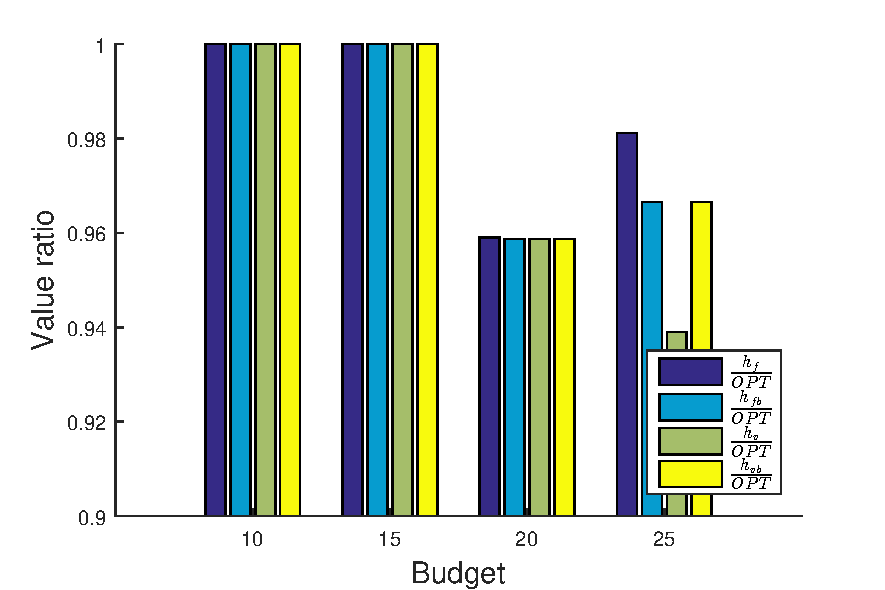
\includegraphics[width=0.48\textwidth]{images/bars_grid_value_ratio}\label{fig:previous_grid_utility}}
\subfigure[Time ratios]
 {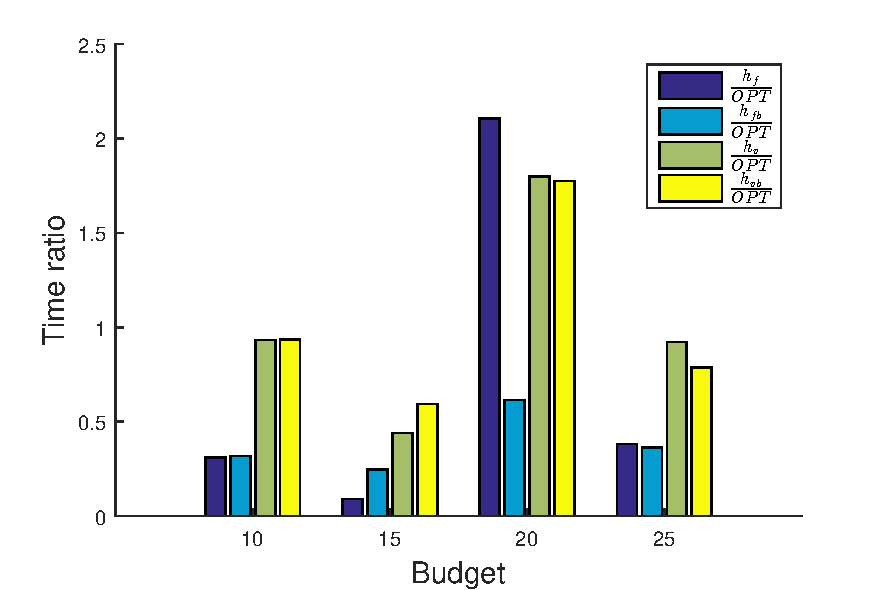
\includegraphics[width=0.48\textwidth]{images/bars_grid_time_ratio}\label{fig:previous_grid_time}}
\caption{Utility and time ratios of PATH w.r.t. FORTIFY on grid graphs.}\label{fig:previous_grid}
\end{figure}

\begin{figure}[!htbp]
\centering
\subfigure[Utility ratios]
  {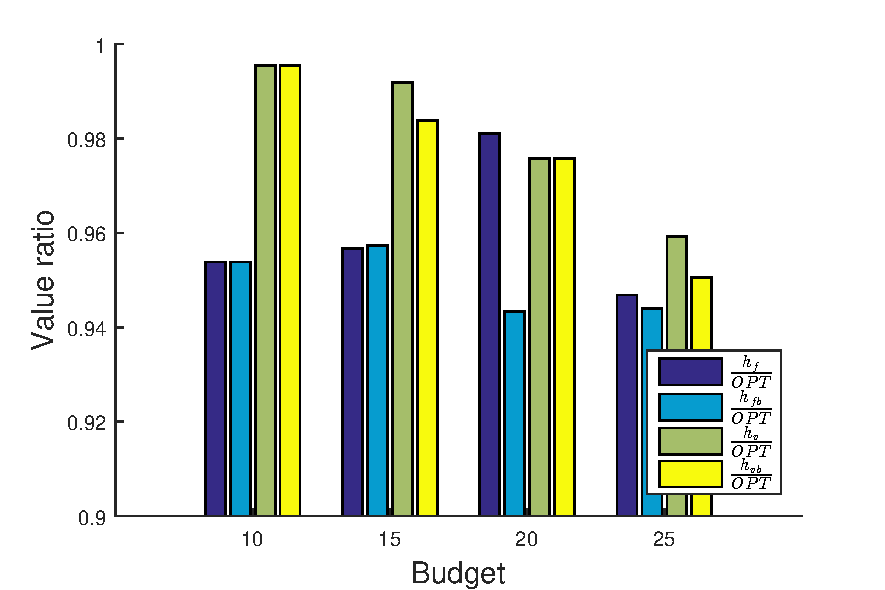
\includegraphics[width=0.46\textwidth]{images/bars_random_value_ratio}\label{fig:previous_random_utility}}
\subfigure[Time ratios]
 {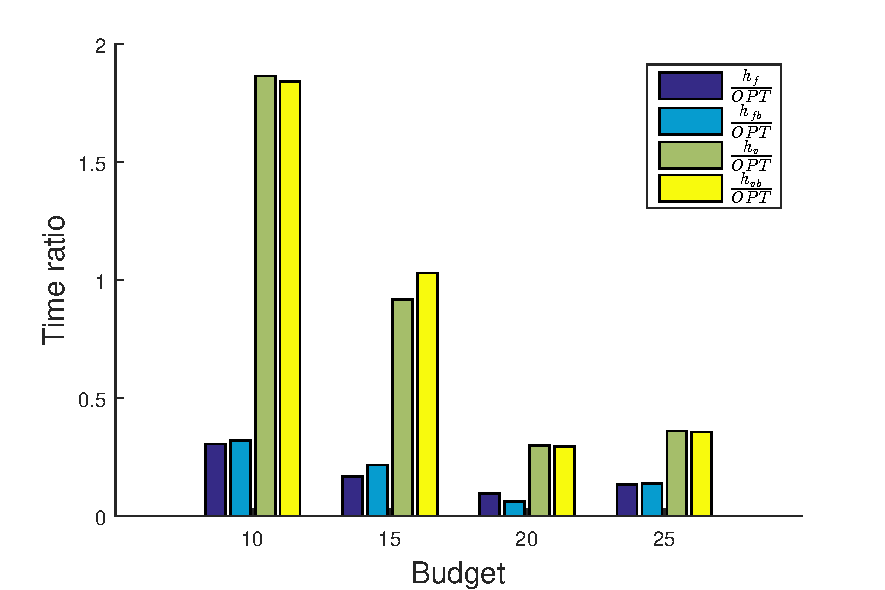
\includegraphics[width=0.46\textwidth]{images/bars_random_time_ratio}\label{fig:previous_random_time}}
\caption{Utility and time ratios of PATH w.r.t. FORTIFY on random graphs.}\label{fig:previous_random}
\end{figure}

\textit{Grid graphs}. Figure~\ref{fig:previous_grid_utility} shows that for low values of the budget, all the heuristics select the same team, getting an approximation ratio higher than 95\% with a budget of 20. If we look at a budget equal to 25, we observe that only $h_v$ is performing worse than the others, but the value is still higher than 94\% of the optimal solution.

Figure~\ref{fig:previous_grid_time} shows the time required by the heuristics w.r.t. the time needed to solve the problem exactly. As we expected, $h_f, h_{fb}$ are faster than $h_v, h_{vb}$, which need to solve the problem also for each single resource. In general, the time required by PATH depends mainly on the time required to solve the exact problem with the team chosen by the heuristic. Thus, depending on the resources the team is composed of and the ways in which such resources can be allocated on the graph, the required time may vary significantly. This explains the (apparently) unusual trends of the time ratios.

%if we include the budget to evaluate the resources, then the resources have the same effectiveness both if we consider their features or the actual value computed solving the problem with such resources as teams of cardinality 1: both methods return an approximation ratio higher than 0.95 as the budget increases. On the other side, if we do not take into account the budget, there is a difference, which is very small: in fact, if we consider the features of the resources, we can provide a utility approximation ratio of 95\% against a worst case of slightly less than 94\% when the budget is equal to 20.

\textit{Random graphs}. Looking at Figure~\ref{fig:previous_random}, we observe that there is a clear difference both in terms of quality solution and computational time for the two main approaches of the heuristics, namely, taking into account the features of the resources or their actual values. Specifically, Figure~\ref{fig:previous_random_utility} shows that, even though the utility ratios are all above 94\%, if we consider the resources according to the utility obtained solving the exact problem, the value computed by the team they chose is higher than the corresponding ones chosen by the other two heuristics. Moreover, the budget does not seem to be a discriminating feature, being $h_f, h_{fb}$ close to each other, and the same holds for $h_v, h_{vb}$. We notice that $h_v$ returns a value equal to 96\% even with a budget of 25.

We focus now on Figure~\ref{fig:previous_random_time}: also in this case, we notice that the budget is not a distinctive feature. Indeed, the times required by $h_f, h_{fb}$ are similar and the same holds for $h_v, h_{vb}$. We observe that for low budgets the time required by the heuristics that adopts the exact values are very high. This is due to the \textit{fixed cost} such heuristics have to pay, namely solving the problem exactly for each resource and then for the chosen team. As the budget increases, FORTIFY requires more and more time because the number of teams to be exactly evaluated grows quickly: our heuristics do not have this issue and consequently, as the budget increases, their time decreases w.r.t. the time required by FORTIFY.


%\subsection{Increasing the size of the graph}\label{sec:synth_size_comp}
%We start increasing the size of the graphs. Specifically, we test SHARD and FORTIFY on the following graphs:
%\begin{itemize}
%\item $R_{25,4,4,r}$ and $r \in \{0.2,0.3\}$;
%\item $R_{30,5,5,r}$ and $r \in \{0.1,0.2,0.3\}$;
%\item $R_{35,6,6,r}$ and $r \in \{0.1,0.2,0.3\}$;
%\item $G_{5,5,s,t}$ with $(s,t) \in \{(2,8),(5,5),(8,2)\}$
%\item $G_{6,6,s,t}$ with $(s,t) \in \{(4,10),(6,6),(10,4)\}$ 
%\end{itemize}
%We employ two sets of resources: $L_1 = \{2,4,5,3,5,6\}, P_1 = \{0.8,0.8,0.8,0.6,0.6,0.6\}, b_1 = \{5,8,10,5,8,10\}$ and $L_2 = \{1,2,3,4,4,6\}, P_2 = \{0.5,0.8,0.7,0.6,0.8,0.9\}, b_2 = \{2,5,8,7,10,12\}$. (We observe that the budget and the number of resources are the same of the previous section).
%
%\subsection{Increasing the budget and the pool of resources}\label{sec:synth_res_comp}
%Here we increase the pool of resources available to $\mathcal{D}$. Specifically, $L = \{1,2,3,4,4,5,5,6,6\}, P = \{0.5,0.8,0.6,0.6,0.7,0.6,0.8,0.6,0.9\}, b = \{2,5,5,7,8,8,10,10,12\}$. We also increase the budget that the Defender can invest to build her team. The graphs we consider are the same of Sec.~\ref{sec:old_synth_comp}.
%
%\subsection{Increasing size, budget and pool of resources}
%Now, we increase our instances along all the three dimensions, considering graphs from Sec.~\ref{sec:synth_size_comp} and resources and budget from Sec.~\ref{sec:synth_res_comp}.

\subsection{Real-world comparison: protecting the Madagascar forests}
We present the following model, which was built working closely with domain experts from NGOs.

\textit{Graph}. We used the road and river networks used by the patrolling officers, as well as the known routes taken by groups of illegal loggers, to build the nodes and edges of our network. Edges correspond to distances of $7$-$10$ km. $10$ target locations were chosen by clustering prominent forest areas. $11$ villages in the surrounding area were chosen as sources. Several domain experts identified the risk level and level of attractiveness for logging, based on the size of the forest, the ease of access and the value of the trees. Using this information we assigned values ranging from $100$ to $300$ to each of the targets.

\textit{Resources pool}. Communal policemen and local volunteers conduct patrols in the forest. A typical patrol covers $20$ km in a day and patroller can conduct two types of patrols, a short patrol covering $2$ edges and a long patrol covering $3$ edges. Based on expert input, we assign the detection probability for communal police as $0.9$ for short patrols and $0.8$ for long patrols; and for volunteers, $0.7$ for short patrols and $0.6$ for long patrols. The lower probabilities for volunteers are because they must call backup for interdiction, which may allow the adversary to escape. Thus, in total we have $4$ resource types available $L = \{2,3,2,3\}, P = \{0.7,0.6,0.9,0.8\}$. The costs are proportional to the salaries patrollers receive for a day of patrolling $b = \{5,5,8,8\}$.

\begin{figure}[!htbp]
\centering
\subfigure[Utility ratios]
  {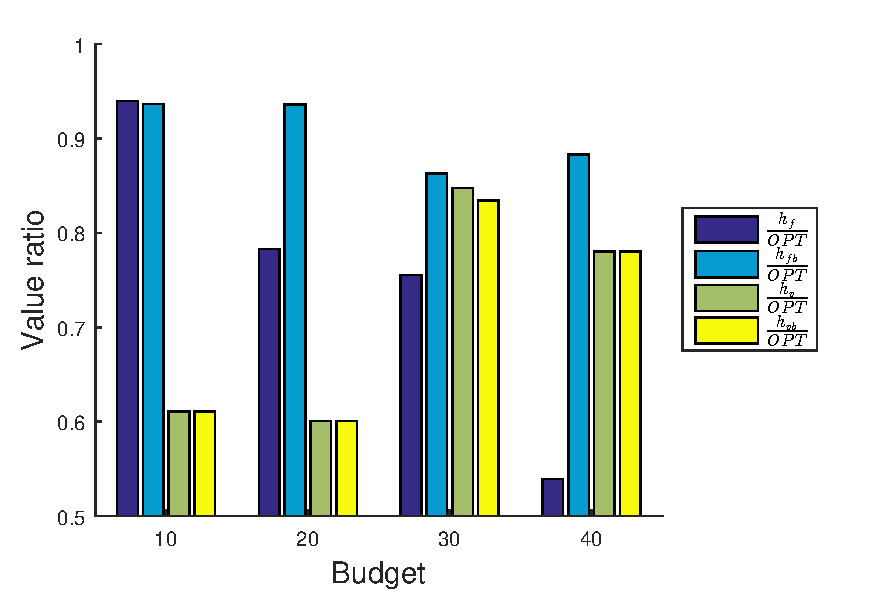
\includegraphics[width=0.46\textwidth]{images/bars_madagascar_value_ratio}\label{fig:previous_madagascar_utility}}
\subfigure[Time ratios]
 {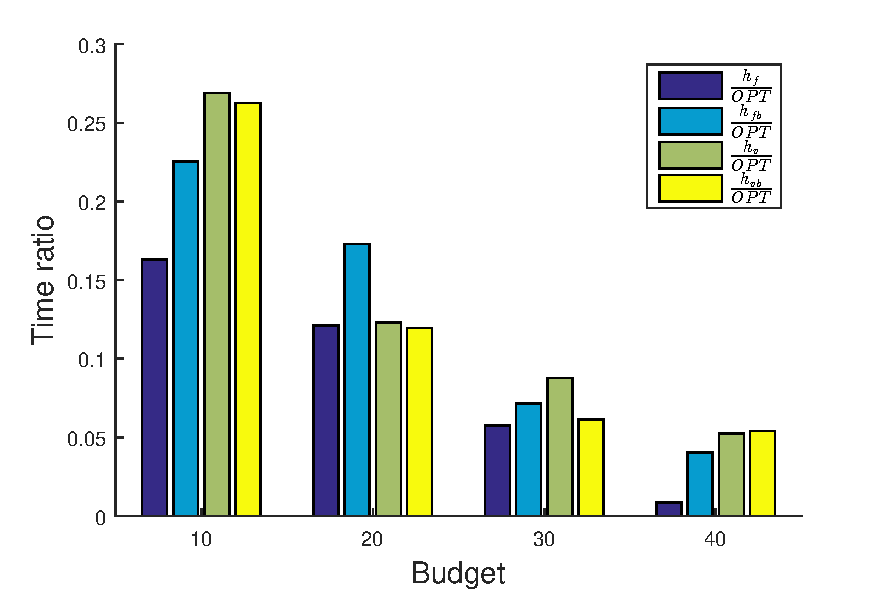
\includegraphics[width=0.46\textwidth]{images/bars_madagascar_time_ratio}\label{fig:previous_madagascar_time}}
\caption{Utility and time ratios of Algorithm~\ref{alg:approximation} w.r.t. FORTIFY on the Madagascar graph.}\label{fig:previous_madagascar}
\end{figure}

\textit{Results}. Differently from the synthetic instances, the results shown in Figure~\ref{fig:previous_madagascar} are apparently contradictory. Indeed, Figure~\ref{fig:previous_madagascar_utility} shows that, for low budgets, $h_v$ and $h_{vb}$ are performing much worse than $h_f, h_{fb}$. The rationale behind this trends is that $h_v$ and $h_{vb}$ form teams with just one type of resource, which results being the best in terms of utility and also the cheapest. As the budget increases, such behavior is mitigated and, adding diversity to the team, the performance improve, reaching also an approximation ratio close to 85\%. While the budget cannot help us in saying whether $h_v$ is always better than $h_{vb}$, it becomes very important when we take into account the features of the resources. In this case, including the budget results being the best behavior, which gives us an approximation ratio higher than 87\% even with a budget of 40. If we focus on Figure~\ref{fig:previous_madagascar_time}, we immediately notice that all the heuristics, independently of the budget, require always less than 30\% of the time employed by FORTIFY. Moreover, the higher the budget, the lower the time ratio. As for Figure~\ref{fig:previous_grid_time}, the apparently unusual trends of such ratio are due to the resolution of the problem for the chosen team.



%\textit{First pool}. Communal policemen and local volunteers conduct patrols in the forest. A typical patrol covers $20$ km in a day and patroller can conduct two types of patrols, a short patrol covering $2$ edges and a long patrol covering $3$ edges. Based on expert input, we assign the detection probability for communal police as $0.9$ for short patrols and $0.8$ for long patrols; and for volunteers, $0.7$ for short patrols and $0.6$ for long patrols. The lower probabilities for volunteers are because they must call backup for interdiction, which may allow the adversary to escape. Thus, in total we have $4$ resource types available $L = \{2,4,2,3\}, P = \{0.7,0.6,0.6,0.5\}$. The costs are proportional to the salaries patrollers receive for a day of patrolling $b = \{5,8,3,5\}$.
%\textit{Results}.

%\textit{Second pool}. Both policemen and volunteers can be enforced either with some sensors and devices, increasing its detection probability, or with vehicles, thus increasing its patrolling capacity, i.e., the number of edges that can be covedered. Thus, the new resources have the following features: $L = \{2,4,4,7,2,3,3,5\}, P = \{0.7,0.6,0.8,0.7,0.6,0.5,0.7,0.6\}, b = \{5,8,10,12,3,5,8,10\}$.
%\textit{Results}.

%Experiment: The runtime experiments are shown in Table 2 for increasing budgets. Data is averaged over 20 runs. FORTIFY can scale up to real world networks, able to handle both the large graph size and number of source and target nodes, even for large budgets. The value of performing this optimization is shown in Figure 7 with the solution quality (game value) on the y-axis and budget on the x-axis, where we compare the optimal game value to the average value achieved by randomly generated teams.

%We present four sets of experimental results: (1) We evaluate the scalability and runtime performance of FORTIFY on several classes of random graphs. We benchmark with a sequential search which sequentially evaluates enumerated teams with cost saturating the budget. (2) We also evaluate the impact of the initial compact layer on the runtime by comparing the runtimes of FORTIFY with and without the compact layer. (3) We investigate the benefit of optimizing team composition as well as the diversity of optimal teams and (4) we demonstrate that FORTIFY can scale up to the real world by testing performance on a case study of Madagascar using real graph data. All values are averaged over 20 trials.
\section{Conclusions and future research}\label{sec:conclusions}
In this work, we studied the problem of preveting illegal logging in developing countries by selecting and allocating at best a team of heterogeneous resources. Due to the rising threat of this problem in South America and Africa, especially in Madagascar, and the limited budget to face this challenge, the selection, coordination and deployment of the available resources become crucial. Due to the vastness of such environments, the approach proposed in the literature is not able to face this problem when either the pool of resources that can be deployed or the budget increase. To deal with this issue, we first provide some results about the team formation problem when the function of the team is submodular. Then, we exploit such results to design a simple but very effective algorithm based on different heuristics. We test our algorithm, showing that the quality of its performance is high while being significantly fast w.r.t. the exact algorithm, allowing us to tackle bigger and closer--to--reality challenges.

In the future, we will expand our research along two dimensions. On one side, we will try to exploit the structure of the graph to improve both FORTIFY and PATH studying possible adaptations of techniques that exploit properties of the graph, e.g., min-cuts or the degree of the nodes. On the other side, we will study scenarios in which resources can be grouped together according to some of their features, e.g., the type of soil they can move on, such as ground, sea or air, making the model more realistic and exploitable for further applications.

%Currently, we are looking for an exact approach that can scale better than FORTIFY. While it is true that the negative results reported here do not encourage us to take such path, they are just posing limits on the exploitation of the team composition. In fact, there is another path that should be explored, namely the structure of the graph. Exploiting such feature could be crucial, and we are tackling this problem on two sides: on one side, we are studying possible adaptations of techniques that exploit min--cuts or other properties of the graph, e.g., the degree of the nodes; on the other, we are investigating flow problems to see if some methods can be adapted to our case.

%In the future, we will study scenarios in which resources can be grouped together according to some of their features, e.g., the type of soil they can move on, such as ground, sea or air, making the model more realistic and exploitable for further applications.

%Moreover, we will also investigate the complimentary problem the one solved in this paper, namely, suggesting how much budget should be invested to guarantee a given level of security.

\newpage

\bibliographystyle{abbrv}
\bibliography{references}

\end{document}







%\title{Instructions for Authors}
%
%\author{} % LEAVE BLANK FOR ORIGINAL SUBMISSION.
%          % UAI  reviewing is double-blind.
%
%% The author names and affiliations should appear only in the accepted paper.
%%
%%\author{ {\bf Harry Q.~Bovik\thanks{Footnote for author to give an
%%alternate address.}} \\
%%Computer Science Dept. \\
%%Cranberry University\\
%%Pittsburgh, PA 15213 \\
%%\And
%%{\bf Coauthor}  \\
%%Affiliation          \\
%%Address \\
%%\And
%%{\bf Coauthor}   \\
%%Affiliation \\
%%Address    \\
%%(if needed)\\
%%}
%
%\begin{document}
%
%\maketitle
%
%\begin{abstract}
%The Abstract paragraph should be indented 0.25 inch (1.5 picas) on
%both left and right-hand margins.  Use 10~point type, with a vertical
%spacing of 11~points.  {\bf Abstract} must be centered, bold, and in
%point size 12. Two line spaces precede the Abstract. The Abstract must
%be limited to one paragraph.
%\end{abstract}
%
%\section{GENERAL FORMATTING INSTRUCTIONS}
%
%Papers are in 2 columns with the overall line width of 6.75~inches
%(41~picas).  Each column is 3.25~inches wide (19.5~picas).  The space
%between the columns is .25~inches wide (1.5~picas).  The left margin
%is 1~inch (6~picas).  Use 10~point type with a vertical spacing of
%11~points.  Times Roman is the preferred typeface throughout.
%
%Paper title is 16~point, caps/lc, bold, centered between 2~horizontal
%rules.  Top rule is 4~points thick and bottom rule is 1~point thick.
%Allow 1/4~inch space above and below title to rules.
%
%Reviewing is double-blind, so do not include author names, affiliations, or any
%other identifying information in the original submission.  If you include urls
%to supplementary material, make sure the urls also do not disclose your identity.
%
%After a paper is accepted, for the camera-ready submission, Authors' names are
%centered, initial caps.  The lead author's name is to be listed first
%(left-most), and the Co-authors' names (if different address) are set to
%follow.  If only one co-author, center both the author and co-author,
%side-by-side.
%
%One-half line space between paragraphs, with no indent.
%
%\section{FIRST LEVEL HEADINGS}
%
%First level headings are all caps, flush left, bold and in point size
%12. One line space before the first level heading and 1/2~line space
%after the first level heading.
%
%\subsection{SECOND LEVEL HEADING}
%
%Second level headings must be flush left, all caps, bold and in point
%size 10. One line space before the second level heading and 1/2~line
%space after the second level heading.
%
%\subsubsection{Third Level Heading}
%
%Third level headings must be flush left, initial caps, bold, and in
%point size 10.  One line space before the third level heading and
%1/2~line space after the third level heading.
%
%\vskip .5pc
%Fourth Level Heading
%
%Fourth level headings must be flush left and initial caps.
%One line space before the fourth level heading and 1/2~line space
%after the fourth level heading.
%
%\subsection{CITATIONS, FIGURES, REFERENCES}
%
%
%\subsubsection{Citations in Text}
%
%Citations within the text should include the author's last name and
%year, e.g., (Cheesman, 1985). Reference style should follow the style
%that you are used to using, as long as the citation style is
%consistent.
%
%For the original submission, take care not to reveal the authors' identity through
%the manner in which one's own previous work is cited.  For example, writing
%``In (Bovik, 1970), we studied the problem of AI'' would be inappropriate, as
%it reveals the author's identity.  Instead, write ``(Bovik, 1970) studied the
%problem of AI.''
%
%\subsubsection{Footnotes}
%
%Indicate footnotes with a number\footnote{Sample of the first
%footnote} in the text. Use 8 point type for footnotes.  Place the
%footnotes at the bottom of the page on which they appear.  Precede the
%footnote with a 0.5 point horizontal rule 1~inch (6~picas)
%long.\footnote{Sample of the second footnote}
%
%\subsubsection{Figures}
%
%All artwork must be centered, neat, clean, and legible. Figure number
%and caption always appear below the figure.  Leave 2 line spaces
%between the figure and the caption. The figure caption is initial caps
%and each figure numbered consecutively.
%
%Make sure that the figure caption does not get separated from the
%figure. Leave extra white space at the bottom of the page rather than
%splitting the figure and figure caption.
%\begin{figure}[h]
%\vspace{1in}
%\caption{Sample Figure Caption}
%\end{figure}
%
%\subsubsection{Tables}
%
%All tables must be centered, neat, clean, and legible. Table number
%and title always appear above the table.  See
%Table~\ref{sample-table}.
%
%One line space before the table title, one line space after the table
%title, and one line space after the table. The table title must be
%initial caps and each table numbered consecutively.
%
%\begin{table}[h]
%\caption{Sample Table Title}
%\label{sample-table}
%\begin{center}
%\begin{tabular}{ll}
%\multicolumn{1}{c}{\bf PART}  &\multicolumn{1}{c}{\bf DESCRIPTION} \\
%\hline \\
%Dendrite         &Input terminal \\
%Axon             &Output terminal \\
%Soma             &Cell body (contains cell nucleus) \\
%\end{tabular}
%\end{center}
%\end{table}
%
%\newpage
%
%\subsubsection*{Acknowledgements}
%
%Use unnumbered third level headings for the acknowledgements title.
%All acknowledgements go at the end of the paper.
%
%
%\subsubsection*{References}
%
%References follow the acknowledgements.  Use unnumbered third level
%heading for the references title.  Any choice of citation style is
%acceptable as long as you are consistent.
%
%
%J.~Alspector, B.~Gupta, and R.~B.~Allen  (1989). Performance of a
%stochastic learning microchip.  In D. S. Touretzky (ed.), {\it Advances
%in Neural Information Processing Systems 1}, 748-760.  San Mateo, Calif.:
%Morgan Kaufmann.
%
%F.~Rosenblatt (1962). {\it Principles of Neurodynamics.} Washington,
%D.C.: Spartan Books.
%
%G.~Tesauro (1989). Neurogammon wins computer Olympiad.  {\it Neural
%Computation} {\bf 1}(3):321-323.
%
%\end{document}
